


\documentclass{beamer}
 
\usepackage[utf8]{inputenc}
\usepackage{siunitx}
\usetheme{CambridgeUS}
\useinnertheme{circles}

\usefonttheme[onlymath]{serif} 
 
%Information to be included in the title page:

\title{Seminar 2}
\subtitle{Overview of astrophysics}

\author{Will Barker\inst{1}\inst{2}}
\institute{
  \inst{1}%
    Cavendish Laboratory\\
    University of Cambridge\\
  \inst{2}%
    Kavli Institute for Cosmology\\
    University of Cambridge\\
}
\date{}
\logo{%
  \makebox[0.95\paperwidth]{%
    
\includegraphics[height=0.7cm,keepaspectratio]{CU.eps}%
    \hfill%
    \includegraphics[height=0.7cm,keepaspectratio]{logo.png}%
  }%
}
 
 
 
\begin{document}
 
\frame{\titlepage}
 
\begin{frame}
  \frametitle{What is astrophysics?}
  \begin{itemize}
    \item $\uparrow$
    \item \textbf{An applied field of physics, so very messy!}
  \end{itemize}
\end{frame}

\begin{frame}
  \center
  \frametitle{Astrophysical phenomena}
  \includegraphics[height=5cm]{kepler_90.jpg}
\end{frame}

\begin{frame}
  \center
  \frametitle{Astrophysical phenomena}
  \includegraphics[height=5cm]{protoplanetary_disk.jpg}
\end{frame}

\begin{frame}
  \center
  \frametitle{Astrophysical phenomena}
  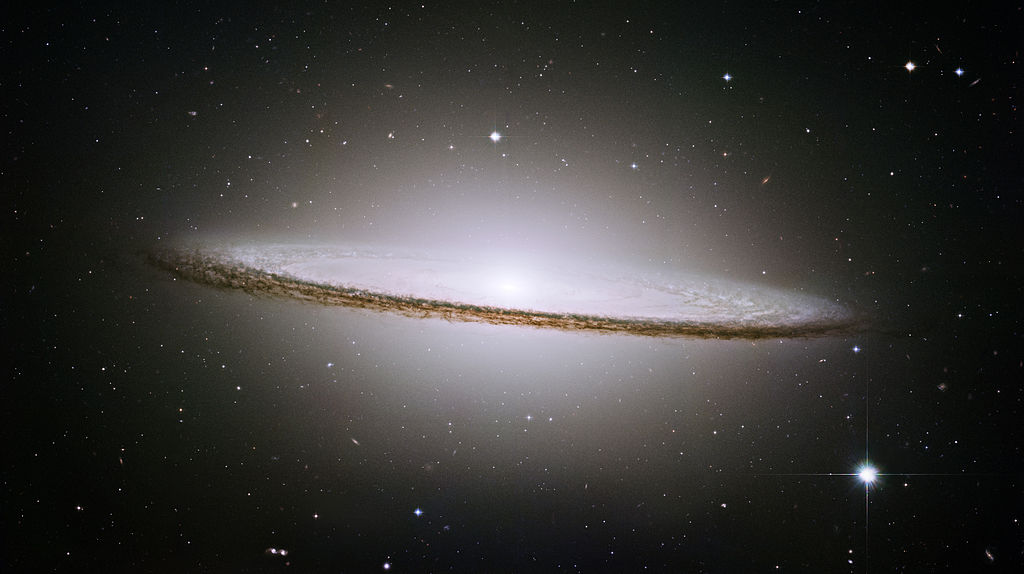
\includegraphics[height=5cm]{sombrero.jpg}
\end{frame}

\begin{frame}
  \center
  \frametitle{Astrophysical phenomena}
  \includegraphics[height=5cm]{m87.jpg}
\end{frame}

\begin{frame}
  \center
  \frametitle{Astrophysical phenomena}
  \includegraphics[height=5cm]{eht.jpg}
\end{frame}

\begin{frame}
  \center
  \frametitle{Astrophysical phenomena}
  \includegraphics[height=5cm]{hl_bh.jpg}
\end{frame}

\begin{frame}
  \center
  \frametitle{Astrophysical phenomena}
  \includegraphics[height=5cm]{gargantua.jpg}
\end{frame}

\begin{frame}
  \center
  \frametitle{Astrophysical phenomena}
  \includegraphics[height=5cm]{lensing.jpg}
\end{frame}

\begin{frame}
  \center
  \frametitle{Astrophysical phenomena}
  \includegraphics[height=5cm]{deep.jpg}
\end{frame}

\begin{frame}
  \center
  \frametitle{Astrophysical phenomena}
  \includegraphics[height=5cm]{cmb.jpg}
\end{frame}

\begin{frame}
  \center
  \frametitle{Astrophysical phenomena}
  \includegraphics[height=5cm]{big_bang.jpg}
\end{frame}

\begin{frame}
  \frametitle{Exoplanet miscellanea}
  \begin{itemize}
    \item We mentioned that transits were not so reliable:
      \includegraphics[height=4cm]{tabby.png}
  \end{itemize}
\end{frame}

\begin{frame}
  \frametitle{Exoplanet miscellanea}
  \begin{itemize}
    \item What is wrong with this light curve?
      \includegraphics[height=4cm]{tabby_2.jpg}
  \end{itemize}
\end{frame}

\begin{frame}
  \frametitle{Exoplanet miscellanea}
  \begin{itemize}
    \item Illustration of multiple \textbf{Dyson rings}:
      \includegraphics[height=4cm]{dyson.png}
  \end{itemize}
\end{frame}

\begin{frame}
  \frametitle{Exoplanet miscellanea}
  \begin{itemize}
    \item HabEx -- atmospheric backlighting in our own solar system:
      \includegraphics[height=4cm]{pluto_atmosphere.jpg}
  \end{itemize}
\end{frame}

\begin{frame}
  \frametitle{Exoplanet miscellanea}
  \begin{itemize}
    \item Which planet, if any?
      \includegraphics[height=4cm]{pluto.jpg}
  \end{itemize}
\end{frame}

\begin{frame}
  \frametitle{Exoplanet miscellanea}
  \begin{itemize}
    \item Solar coronograph:
      \includegraphics[height=4cm]{coronograph.png}
  \end{itemize}
\end{frame}

\begin{frame}
  \frametitle{Astrophysical scale}
  \begin{itemize}
    \item By definition, astrophysics will involve a wide range of \textbf{length scales}
  \end{itemize}
\end{frame}

\begin{frame}
  \frametitle{Astrophysical scale}
  \begin{itemize}
    \item Distance to space: \SI{1e2}{km}
  \end{itemize}
\end{frame}

\begin{frame}
  \frametitle{Astrophysical scale}
  \begin{itemize}
    \item Distance to the moon: \SI{4e5}{km}
  \end{itemize}
\end{frame}

\begin{frame}
  \frametitle{Astrophysical scale}
  \begin{itemize}
    \item Before we proceed further, we need to get to grips with the speed of light\ldots
  \end{itemize}
\end{frame}

\begin{frame}
  \frametitle{Astrophysical scale}
  \begin{itemize}
    \item The speed of light $c$ has the value \SI{3e8}{m/s}
    \item The earth has radius \SI{6.4e6}{m}, so how many times would light travel around the earth?
    \item The speed of light is \textbf{fixed}, it doesn't matter how you change you own velocity, $c$ will always give the same value upon measurement
  \end{itemize}
\end{frame}

\begin{frame}
  \frametitle{Astrophysical scale}
  \center
  \includegraphics[height=7cm]{mm.png}
\end{frame}

\begin{frame}
  \frametitle{Astrophysical scale}
  \begin{itemize}
    \item Counter-intuitively $c$ has \textbf{nothing} to do with light or electromagnetism, rather it is a unit-conversion between \textbf{space} and \textbf{time} -- which as we will see in Seminar 4 and 5, are the same thing
    \item Field theories (such as electromagnetism) have a mathematical structure such that (at the level of QFT) they contain \textbf{massless particles}
    \item \textbf{Special relativity} tells us that massless particles \textbf{always} move at $c$, or for every bit of time which elapses, they move through an \textbf{equal} bit of space
    \item \textbf{massive particles} (such as yourselves!) are free to move at any speed below $c$
  \end{itemize}
\end{frame}

\begin{frame}
  \frametitle{Astrophysical scale}
  \begin{itemize}
    \item Electromagnetism and quantum electrodynamics are not unique in that they contain massless \textbf{photons}
    \item Quantum chromodynamics (strong force) contains massless \textbf{gluons} and \textbf{classical} theories of gravity predict \textbf{gravitational waves} moving at $c$
    \item We expect that any quantum theory of gravity would therefore contain a massless \textbf{graviton}
  \end{itemize}
  \center
  \includegraphics[height=2cm]{gluon.png}
\end{frame}

\begin{frame}
  \frametitle{Astrophysical scale}
  \begin{itemize}
    \item \ldots back to astrophysics: because $c$ is so large, it is fairly useful for talking about scale
    \item The light minute: \SI{1.8e7}{km}
    \item The light year: \SI{9.5e12}{km}
    \item Clearly we are now talking about vast distances
  \end{itemize}
\end{frame}

\begin{frame}
  \frametitle{Astrophysical scale}
  \begin{itemize}
    \item Distance to the sun: \SI{8.5}{lm}
    \item Distance to the edge of the solar system: \SI{1}{ld}
    \item Let's pause here to define the \textbf{parsec}:
      \begin{itemize}
	\item The distance at which one \SI{1}{au} subtends one \textbf{arcsecond}
      \end{itemize}
  \end{itemize}
\end{frame}

\begin{frame}
  \frametitle{Astrophysical scale}
  \begin{itemize}
    \item Moving out\ldots
    \item Distance to Proxima Centauri: \SI{4.2}{ly}
    \item Distance to TRAPPIST-1: \SI{40}{ly}
    \item Distance to Sag A*: \SI{2.6e4}{ly}
    \item From this we get the length scale of our galaxy: \SI{1e4}{ly}
  \end{itemize}
\end{frame}

\begin{frame}
  \frametitle{Astrophysical scale}
  \begin{itemize}
    \item Since I mentioned Proxima b:
      \begin{itemize}
	\item https://www.youtube.com/watch?v=lysJduOqads 
	\item https://www.youtube.com/watch?v=RoCm6vZDDiQ
      \end{itemize}
  \end{itemize}
\end{frame}

\begin{frame}
  \frametitle{Astrophysical scale}
  \begin{itemize}
    \item Distance to LMC and SMC: \SI{1e5}{ly}
    \item Distance to Andromeda galaxy: \SI{2.5e6}{ly}
    \item Distance to M87: \SI{16.4e6}{pc}
  \end{itemize}
\end{frame}

\begin{frame}
  \frametitle{Astrophysical scale}
  \begin{itemize}
    \item Finally distance to the edge of the known universe: \SI{14e9}{pc}
  \end{itemize}
\end{frame}

\begin{frame}
  \frametitle{Astrophysical scale}
  \begin{itemize}
    \item Once we are in the realm of \SI{1e6}{pc} we should really be talking about \textbf{redshift}
    \item You will have heard about redshift in the context of fast-moving objects
    \item When we observe distant galaxies, we find that redshift \textbf{increases} with distance, and furthermore it does so \textbf{linearly} -- this is \textbf{Hubble's Law}
    \item The observed redshift indicates that distant objects are moving \textbf{away from us} at a rate known as $H$, the Hubble constant
  \end{itemize}
\end{frame}

\begin{frame}
  \frametitle{Astrophysical scale}
  \center
  \includegraphics[height=7cm]{hubbel.png}
\end{frame}

\begin{frame}
  \frametitle{Astrophysical scale}
  \begin{itemize}
    \item Early estimates based on both CMB and light geodesics agree
    \item More recently they are diverging, so-called \textbf{Hubble tension}
    \item Evidence perhaps that \textbf{general relativity is lacking\ldots}
  \end{itemize}
\end{frame}

\begin{frame}
  \frametitle{Astrophysical scale}
  \begin{itemize}
    \item To see what this has to do with redshift, we need to understand how light moves through an expanding universe
    \item Easiest with \textbf{plane-polar coordinates}, $r$ and $\phi$
    \item In Euclidean space take $r$ to be dimensionful, $\phi$ dimensionless
    \item Then add dimensionful time $t$, and re-parameterise the radial coordinate with dimensionful $R(t)$ and dimensionless $r$
  \end{itemize}
\end{frame}

\begin{frame}
  \frametitle{Astrophysical scale}
  \begin{itemize}
    \item Euclidean case:
      \begin{equation*}
	v^2\mathrm{d}t^2-\mathrm{d}r^2-r^2\mathrm{d}\phi^2=0,\quad c^2\mathrm{d}t^2-\mathrm{d}r^2-r^2\mathrm{d}\phi^2=0
      \end{equation*}
    \item Non-Euclidean case:
      \begin{gather*}
	v^2\mathrm{d}t^2-R(t)^2\mathrm{d}r^2-R(t)^2r^2\mathrm{d}\phi^2=0,\\
	c^2\mathrm{d}t^2-R(t)^2\mathrm{d}r^2-R(t)^2r^2\mathrm{d}\phi^2=0
      \end{gather*}
  \end{itemize}
\end{frame}

\begin{frame}
  \frametitle{Astrophysical scale}
  \begin{itemize}
    \item Time-permitting, an asside on \textbf{proper time} vs \textbf{coordinate time}\ldots
  \end{itemize}
\end{frame}

\begin{frame}
  \frametitle{Astrophysical scale}
  \begin{itemize}
    \item So now we know how light behaves in an expanding universe:
      \begin{equation*}
	c^2\mathrm{d}t^2-R(t)^2\mathrm{d}r^2=0 \implies \frac{c\mathrm{d}t}{R(t)}=\mathrm{d}r	
      \end{equation*}
    \item We can take this and \textbf{integrate} over the passage of a light wave from \textbf{early} $t_1$ to \textbf{contemporary} $t_0$:
      \begin{equation*}
	\frac{\delta t_1}{R(t_1)}=\frac{\delta t_0}{R(t_0)}
      \end{equation*}
  \end{itemize}
\end{frame}

\begin{frame}
\frametitle{Astrophysical scale}
  \begin{itemize}
    \item Now we get to re-express this in terms of wavelength, frequency etc:
      \begin{equation*}
	c\delta t_1=\lambda_1, \quad c\delta t_0=\lambda_0	
      \end{equation*}
    \item Define the redshift (should be $z>0$ for an \textbf{expanding} universe):
      \begin{equation*}
	z=\frac{\lambda_0}{\lambda_1}-1	
      \end{equation*}
    \item So finally we have:
      \begin{equation*}
	\frac{\delta t_1}{R(t_1)}=\frac{\delta t_0}{R(t_0)}\implies z+1=\frac{R(t_0)}{R(t_1)}
      \end{equation*}
  \end{itemize}
\end{frame}

\begin{frame}
  \frametitle{Astrophysical scale}
  \begin{itemize}
    \item Hence, redshift depends on the size of the universe at emission and detection
    \item If the universe is \textbf{matter dominated} general relativity suggests $R(t)\propto t^{2/3}$
    \item Try to find the observed age of these galaxies in the matter dominated universe, given $t_0$ is \SI{1.4e10}{yr}:
      \begin{itemize}
	\item M87 at $z=0.00428$
	\item Sombrero galaxy at $z=0.003416$
	\item GN-z11 at $z=11.09$
      \end{itemize}
  \end{itemize}
\end{frame}

\begin{frame}
  \frametitle{Astrophysical scale}
  \begin{itemize}
    \item Main point is that the most distant \textbf{observable} objects are significantly further away than light could have travelled over the entire age of the universe
  \end{itemize}
\end{frame}

\begin{frame}
  \frametitle{Astrophysical scale}
  \center
  \includegraphics[height=7cm]{gn_z11.jpg}
\end{frame}

\begin{frame}
  \frametitle{Astrophysical scale}
  \begin{itemize}
    \item Hopefully we will get on to some astrophysical fluid dynamics, but we need \textbf{vector calculus} to do that
  \end{itemize}
\end{frame}

\begin{frame}
  \frametitle{Astrophysical scale}
  \begin{itemize}
  \end{itemize}
\end{frame}
\end{document}


